\section{Overall architecture}\label{sec:mira-microcity}

As mentioned in the previous section, Mirabilandia does not offer a recommendation or virtual queuing services.
In this section, we describe a possible implementation of the "smart micro-city" concept applied to the context of amusement parks, specifically that
of Mirabilandia.

\begin{figure}[H]
	\centering
	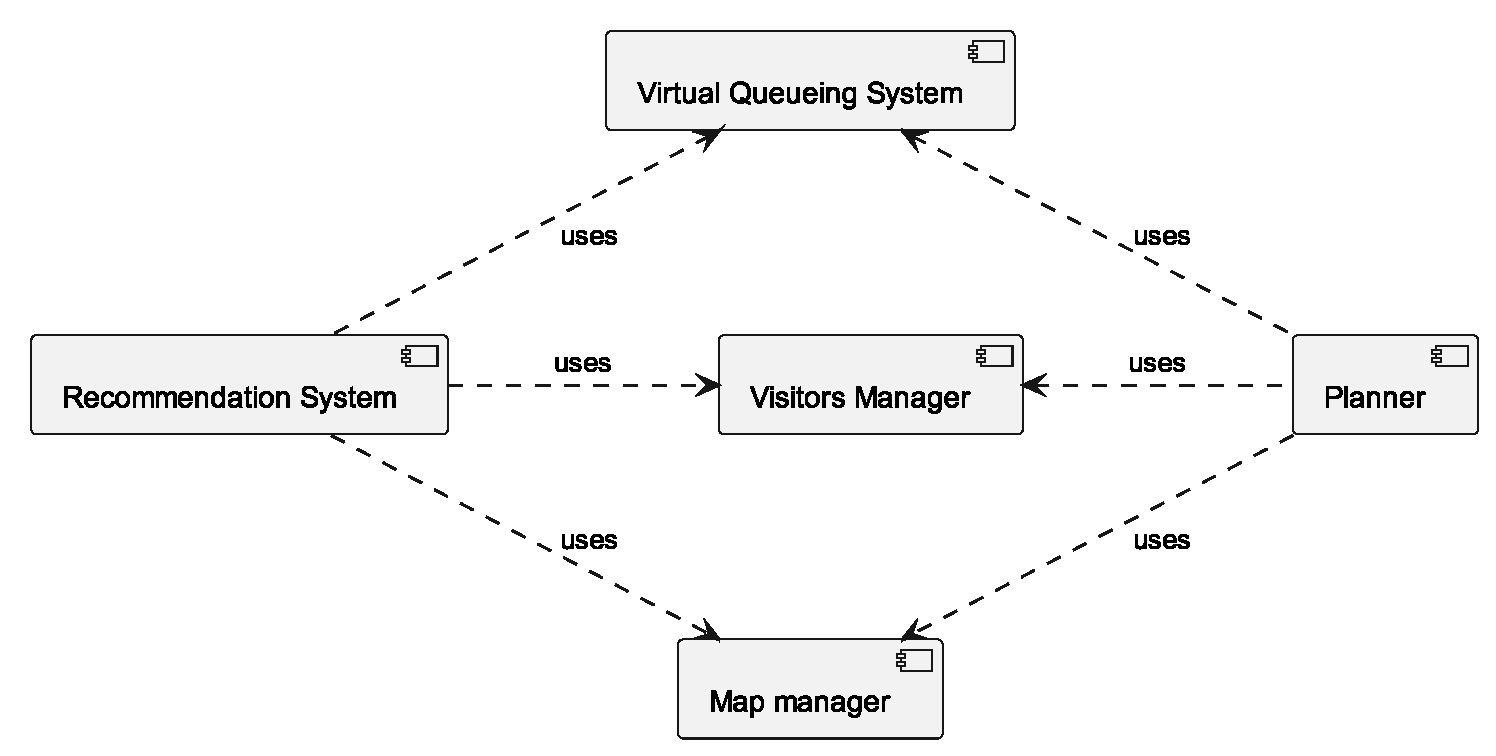
\includegraphics[width=0.9\textwidth]{img/architecture-overview.eps}
	\caption{Overview architecture of Mirabilandia as a micro-city.
		The component diagram shows the rough architecture in the context of Mirabilandia, showing the main dependencies between them.
	}
	\label{fig:architecture-overview}
\end{figure}

Following the analysis of the ``as-is'' system and the goals set to adapt the smart micro-city concept on Mirabilandia,
figure~\ref{fig:architecture-overview} shows the component diagram modeling the entities involved and the main relationships between them.

The main components of the system are the following:

\begin{itemize}
	\item \textit{Map Manager}: is responsible for tracking the guest within the park and providing information about the current position
	\item \textit{Virtual Queueing System}: is responsible for managing the virtual queue for each attraction
	\item \textit{Recommender}: is responsible for providing recommendations to the guests based on their preferences and position within the park
	\item \textit{Planner}: is responsible for planning the itinerary of the guests based on their preferences and crowding of rides
\end{itemize}

From the diagram emerge that \textit{Map Manager} and \textit{Virtual Queueing System} are the main components of the system since they are the ones
that provide information to the other components. The \textit{Map Manager} provides information about the current position of the guests
to the \textit{Recommender} which uses this information to provide recommendations to the guests. Moreover, gives information also to the
\textit{Planner} to avoid crowd situations and maintain a uniform distribution of guests in the park. The \textit{Virtual Queueing System} is used by
the \textit{Planner} to plan the itinerary of the guests and adapt it to reduce the waiting time and improve the quality of the visit within the park
and by the \textit{Recommender} to fetch information about the current waiting time of the attractions and opportunistically advise the attraction.

\section{Map Manager}

The location of guests within the amusement park is critical for several reasons: guest location information is used to make recommendations and to determine the best plan for each guest. So, good tracking is crucial for the good working of the overall system.

\begin{figure}[H]
	\centering
	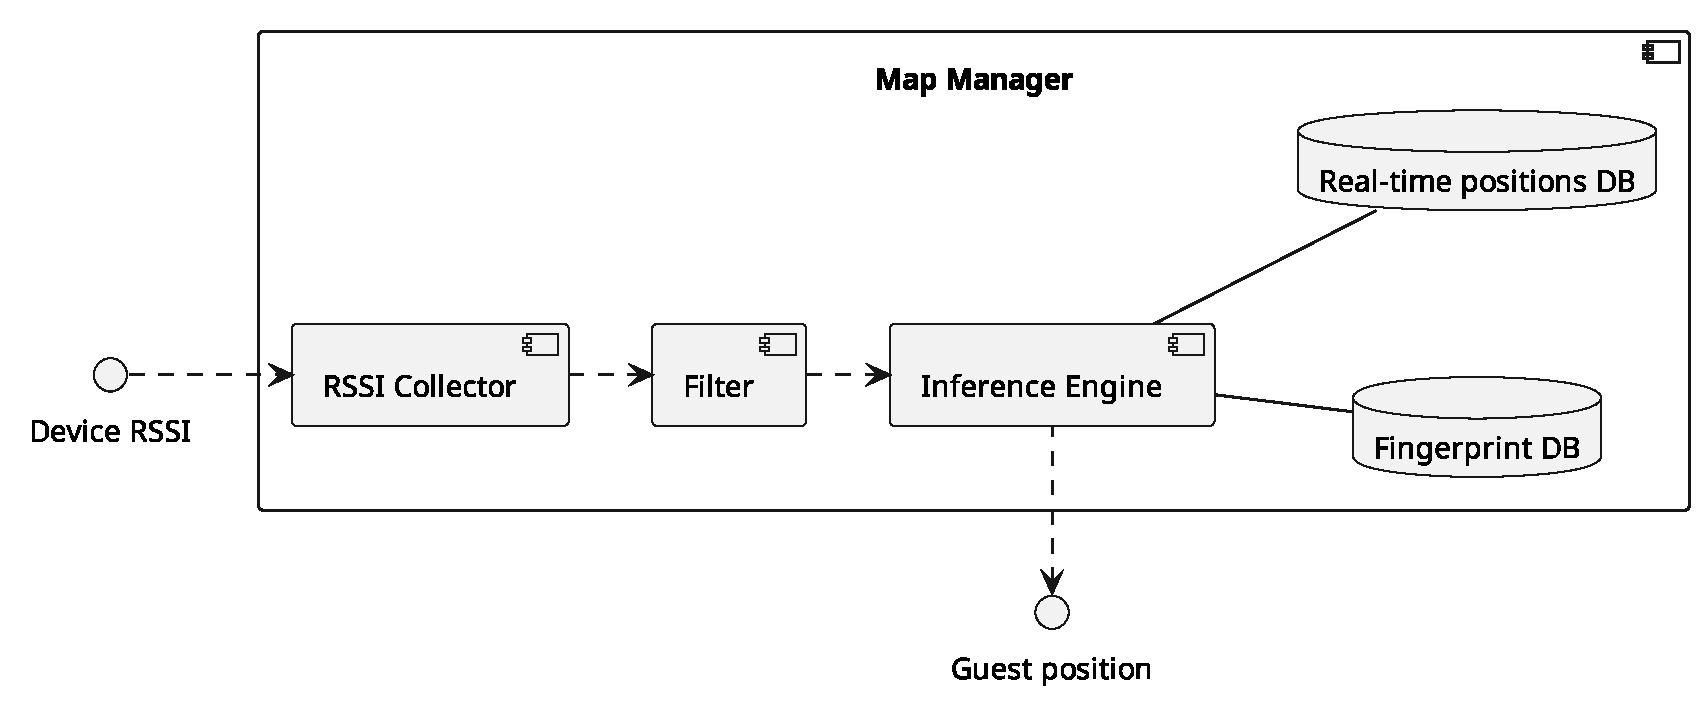
\includegraphics[width=\textwidth]{img/map-manager.eps}
	\caption{Component diagram showing the internal architecture of the \textit{Map Manager} component.
	}
	\label{fig:map-manager}
\end{figure}

\subsection{Technologies for visitors localization}\label{sec:technologies}
Visitors localization could be useful for both proximity marketing and calculating the number of people in a queue.
Indoor localization could be helpful in our context as there are restaurants, shops and some attractions
(e.g.\ Reset\footnote{\url{https://www.mirabilandia.it/en/attivita/attrazioni/reset}}) not easily reached by the outdoor localization technologies.
Moreover, the accuracy of outdoor localization technologies (e.g.\ GPS) may not be enough accurate for instance for the prize games area\footnote{\url{https://www.mirabilandia.it/en/attivita/attrazioni/altri-giochi-e-giochi-a-premio}}
where the stands are located next to each other.

To design and develop an effective technique for the location of visitors, the following constraints were considered:
\begin{itemize}
	\item The use of a custom device is not feasible since most people reject the use of a custom device. Using each visitor's device would
	      be a better choice because they do not have the impediment of an extra device and do not need any training to use it
	\item The use of dedicated hardware results in an extra cost that is difficult for both the amusement park and visitors to bear.
\end{itemize}

Some technologies identified for these purposes will be described in the following sections, taking into account the constraint defined above.

\subsubsection{Wi-Fi as outdoor localization system}\label{subsec:wi-fi-as-outdoor-localization-system}

Wi-Fi is a family of wireless network protocols, which are commonly used for local area networking of devices and Internet access, allowing the nearby digital device to exchange data by radio waves.

To date, Wi-Fi is a technology that has been pervasively adopted and made accessible to anyone because of cost, ease of installation and configuration.

Unlike other technologies such as the global positioning system (GPS), Wi-Fi was not designed to perform device and/or person location.
However, by exploiting ad-hoc techniques it is possible to leverage this tool to perform device localization.
Finally, GPS does not always perform well in any context: in closed environments or where the GPS signal cannot reach, localization using
this technology is approximate or even impractical.
Another problem with GPS is its high power consumption, which is a serious challenge to battery-based mobile devices.
To tackle the problems with GPS, many researchers have proposed a series of alternative localization schemes, including cellular-based
systems~\cite{ibrahim2010cellsense}, infrared-based systems, ultrasonic-based systems, and radio frequency (RF)-based
systems~\cite{bahl2000radar, youssef2002probabilistic}.

Many researchers have proposed a variety of different schemes for outdoor localization based on mobile devices.
These schemes can be divided into two groups: range-based and range-free methods.

\begin{itemize}
	\item \textbf{Range-based}: range-based methods are mainly based on relative distance, which can be obtained through measuring methods like
	      time-of-arrival (ToA), time difference of arrival (TDoA), or propagation model generated from RSSI value.
	\item \textbf{Range-free}: one of the most widely used range-free methods is the fingerprint localization method.
	      This method can be categorized into three types:
	      visual fingerprint-based localization, motion fingerprint-based systems, and signal fingerprint-based methods.
	      In our context, the latter is the most promising.
\end{itemize}

\subsubsection{Signal fingerprint-based localization}
Signal fingerprint-based localization is widely used in places where a large number of Wi-Fi infrastructures are deployed.
This method commonly consists of an offline training phase and an online fingerprint matching phase.
The goal of the first phase is to form a fingerprint database that stores the correlation between \textit{Received Signal Strength} (RSS) from
various \textit{Access Points}(APs) and fixed locations. The device's location is determined at the matching stage.
In this process, we use a matching algorithm to search the fingerprint in the database which has the minimum difference with the device that needs to
be located. The associated label is our estimated location.

\subsubsection{Signal fingerprint-based localization improvement with NFC technology}
In terms of effect, signal fingerprint-based localization can get fine-grained results.
However, as any radio environment is dynamic: unpredictable movements of the people or large unforeseen gatherings,
alterations in the radio network itself, environmental effects such as a change in humidity levels etc.~\cite{chaudhry2013indoor}
Therefore, the RF values measured for location estimation at any given point in time may significantly deviate from
those stored in the database created at the training phase~\cite{chaudhry2013indoor}.
As a result, the location estimation based on a static database may be inaccurate.
Also, the training phase needs a human operator (or a human-assisted machine) to thoroughly collect the RF context and
the location from which the context was collected.
To tackle these problems, as suggested in~\cite{chaudhry2013indoor}, could be useful a system that considers the NFC technology:
reference points of precisely known locations are spread in the environment, marked by NFC tags, to build the database of fingerprints around.
This could improve the training phase and allows easy adaptation to environmental changes.

\subsubsection{Bluetooth as outdoor localization system}
Bluetooth is a data transmission standard for personal wireless networks. It provides a standard way to exchange information between
devices through a short-range frequency capable of detecting devices covered by the radio signal within about ten meters by putting them
in communication with each other.

Despite being a technology conceived more than 20 years ago, it boasts massive adoption in many contexts such as medical, industrial, and in
recent years the Internet of Things (IoT). This standard was designed to achieve low power consumption, short range
and a low cost of production. Over the years, there have been several updates to the protocol, aimed at improving on the one hand the efficiency of
communication by enabling higher transmission frequencies and on the other hand improving the energy efficiency of devices.

Bluetooth was not designed to perform localization functionality. However, it is possible to exploit certain
features of the protocol to make a more or less precise estimate of a device's location. In particular, the technique most
used to achieve this is based on the signal strength identified by the RSSI (Receives Signal Strength Indicator).
Other techniques, such as fingerprint-based localization can be employed to estimate position.

With the RSSI-based technique, the RSSIs of all reachable Bluetooth devices are initially acquired, and through techniques of trilateration, the
location of the device is estimated.\\
Fingerprint-based techniques estimate the location by operating in two stages: the first is the training phase that deals with building fingerprints,
which is a record that associates a location with the RSSIs of beacons reachable from that point.
The second phase involves identifying the fingerprint that least deviates from the position where the device is at a given time, and the
position associated with that fingerprint determines the estimated position. Several projects and applications rely on these two techniques to
estimate the position of a device~\cite{mcconville2021vesta, samuel2021smart}.

The proliferation of location services for various IoT applications needs to detect device locations with very high accuracies, on the order of
centimeters. With the introduction of the Bluetooth 5.1 standard, a new feature called \textit{Direction Finding} enables pinpoint localization
of Bluetooth devices.
This new localization feature provides two different options for positioning a Bluetooth device, namely Angle of Arrival (AoA) and Angle of Departure
(AoD) compared to the previous version that relies only on the received signal strength indication to localize a Bluetooth device.
To be more precise, the former technique allows a receiver equipped with a multi-antenna array to identify the angular position of a transmitter
based on the phase delay of the signal received from the transmitter; the latter allows the transmitting device with multiple antennas to transmit a
radio signal that permits the receiver to determine the directional angle to the transmitter.

\subsection{Suitable localization techniques for Mirabilandia}
In this section, we will discuss the suitability of the localization techniques described in the previous section for Mirabilandia.

Given its size and organization, it comes naturally to think of Mirabilandia as a micro-city: streets, avenues and squares define the street network
that connects all the park's attractions and activities, just as it does for any full-scale city. The arrangement of buildings around
the streets also makes Mirabilandia a micro-city.

Given the similarities to a full-size city, we can assume with some degree of confidence that the amusement park environment is almost identical to
the city environment.
Therefore, we assume that the noise and electromagnetic pollution are quite similar, and therefore all the considerations made in the previous
sections apply.

There is no definite information on the spread and coverage of Wi-Fi within the park, however, it is possible to assume that there is.
Conversely, it is by no means a given that there are Bluetooth devices that can act as beacons.
In light of these considerations, we found that localization using Wi-Fi is the most reasonable in terms of both effectiveness and cost of
installation and configuration. The choice of using Wi-Fi as a technology to support visitor tracking is based on three main considerations:

\begin{itemize}
	\item The cost of installation and configuration is relatively low since we have assumed a partially available infrastructure
	\item The spread of the technology is relatively wide, so any visitor's device support this technology.
	\item The literature about localization using Wi-Fi is relatively large, so it is feasible to use this technology.
\end{itemize}

In this scenario, Bluetooth technology has been discarded because of the low signal range and this would force the installation of many more devices
than would be needed by taking advantage of Wi-Fi; also because in outdoor environments Bluetooth provides lower guarantees in terms of signal
stability and this results in possible inaccuracies in location estimation.
Finally, the introduction of the 5.1 standard is fairly new, and while it is not a problem in terms of adoption, there are still no comprehensive
studies on its effectiveness in amusement park-like environment.

Below we will illustrate a possible technique for implementing park visitor tracking by exploiting Wi-Fi as a supporting technology.
The development of this technique is based on work done by~\cite{du2018hybrid}~and~\cite{chaudhry2013indoor}.

The localization scheme consists of three main phases:

\begin{itemize}
	\item \textbf{Training phase:} in this phase, the system collects the RSSI values of the Wi-Fi APs in the park and associates them with a
	      physical position. This phase could be performed by a human operator or a human-assisted machine
	\item \textbf{Tiling phase:} in this phase the system divides the park into a grid of tiles and caches the values belonging to it
	\item \textbf{Inference phase:} in this phase the system calculates the dissimilarity between the collected patterns and the sample
	      patterns in the database built before. The location of the fingerprint with the minimum difference will be selected as an estimation for the
	      location of the device.
\end{itemize}

The \textit{training phase} is the most important and challenging phase of the scheme. It is the phase in which the system collects the RSSI values
of the Wi-Fi APs in the park and associates them with a physical position. The accuracy of this phase is crucial: a wrong position in a fingerprint
could result in inaccurate location estimation. The collection of the fingerprint database could be done in several ways: by a human operator, which
walking around the park collects the RSSI values of the Wi-Fi APs and associates them with a physical position, creating a fingerprint record.
Alternatively, a fleet of robots (like drones) could be used to collect the RSSI values and associate them with a physical position. This scenario
is ambitious but could be faster and less error-prone than the human ones.

The \textit{tile phase} consists of a series of optimizations exploited by the \textit{inference phase} to reduce the inference time.
The map is divided into regions, each containing fingerprints of the locations contained in it.
In this way, it is not required to use the entire fingerprint database, but only the region (or regions) of interest.
Finally, each tile can be cached for additional performance improvements during the inference phase.
Determining which tile should be used for the inference step is not an easy task. Choosing the wrong tile may result in an incorrect
position estimate. At the same time, it is particularly inefficient to estimate the position by leveraging the entire fingerprint database.
For this reason, a sensor-assisted matching method can restrict the matching operation in a small space through sensor information including
direction and travel distance. The current location can be calculated from an initial location, which can be taken from the GPS, for example.
The distance and direction can be estimated using the dead reckoning~\footnote{\url{https://en.wikipedia.org/wiki/Dead_reckoning}} method with
built-in inertial sensors like accelerometer, gyroscope, and compass.
Given the longitude and latitude of the start point, the distance and bearing from the start point, and the destination point can be calculated using
the Haversine formula~\footnote{\url{https://en.wikipedia.org/wiki/Haversine_formula}}. In this way, a subset of the local fingerprint database cache
can be obtained.

The \textit{inference phase} is the most important phase of the scheme. It is the phase in which the system calculates the position of the device.
Let's denote by $f = {r_1, r_2, \ldots, r_n}$ a \textit{fingerprint} record where $r_i$ represents the RSS value of captured AP and $n$ the number of
APs in the fingerprint record.
Let's calculate the dissimilarity between two fingerprints based on the RSSI difference.
Denote with $\sigma_i = | r_i - r^{'}_{i}|$ the difference of fingerprints $f^{'}$ and $f$ at each $A_i$ where $A_i \in A$ where $A$ is the
fingerprint's APs set.
Since two fingerprints may contain a different set of APs, the access point $A_i$ may appear in $f$ but does not appear in $f^{'}$.
For this situation, we assume the signal strength is weak and let the missing value equal to $-100$.
The dissimilarity between $f$ and $f^{'}$ is calculated via the following formula:

\begin{equation}
	\eta(f, f^{'}) = \sqrt{\sum_{i=0}^{p} \sigma_i^{2}}
	\label{eq:dissimilarity}
\end{equation}

where $p = | A \cup A^{'} |$

The location is calculated via the sample with minimum dissimilarity by comparing all samples stored in the fingerprint database $F$ with the query
fingerprint $f$.

\begin{equation}
	f^{*} = \arg \min_{f_i \in F} \ \eta(f, f_i)
	\label{eq:min-dissimilarity}
\end{equation}

$L(f^{*})$ is the corresponding location of $f^{*}$ which represents the estimated place.

As can be seen from formula~\ref{eq:min-dissimilarity}, the iteration over all fingerprints cannot scale at all: the time needed to iterate all
the fingerprints are proportional to the number of them. In large maps, the number of fingerprints could become very huge degrading the inference
time. It is in this situation that tiling improves performance due to dimension reduction; this reduction is determined by the $k$ factor, where
$k$ is the number of tiles of the map.

\begin{figure}[H]
	\centering
	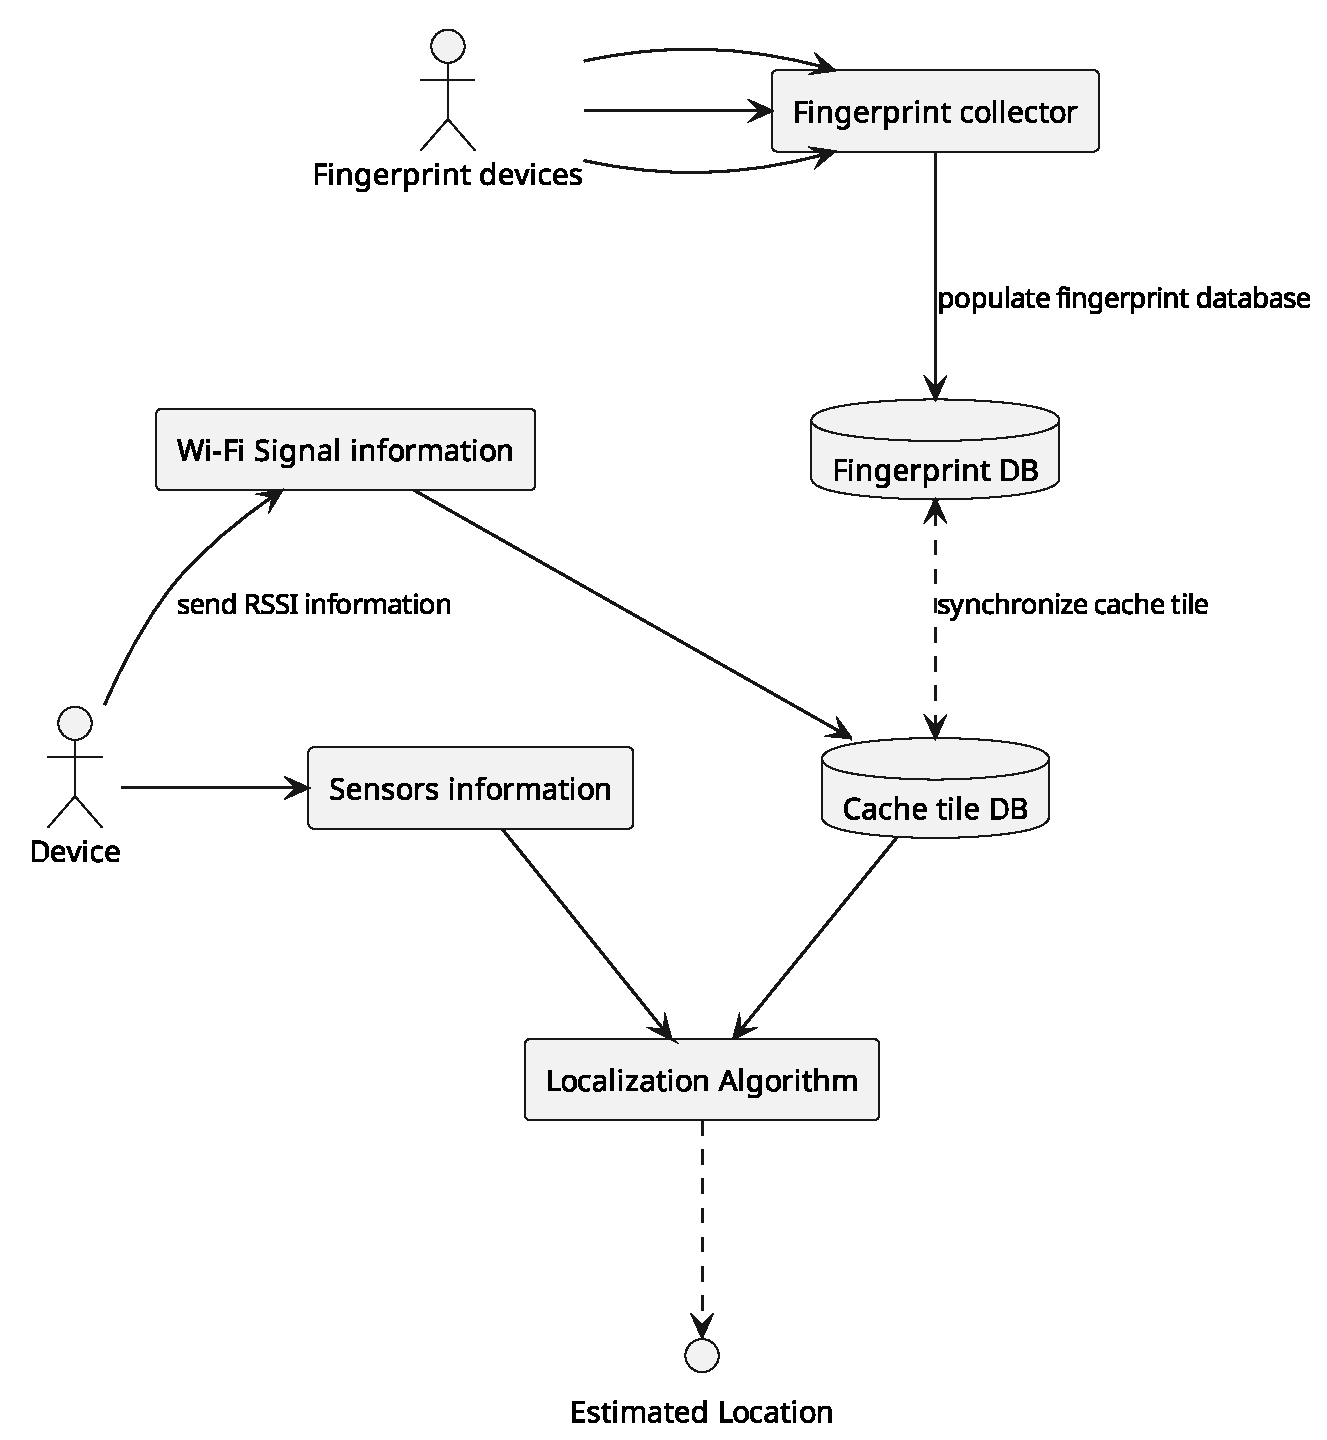
\includegraphics[width=0.7\textwidth]{img/fingerprint-schema.eps}
	\caption{Main steps in the proposed schema for Wi-Fi fingerprint-based localization technique.}
	\label{fig:fingerprint-schema}
\end{figure}

In figure~\ref{fig:fingerprint-schema} are summarized the steps for the localization based on Wi-Fi.

The adoption of this technique leads to several advantages:
\begin{itemize}
	\item The accuracy of the localization is improved compared with the GPS one~\cite{du2018hybrid}
	\item The power consumption needed to implement this system is sensible lower than the GPS~\cite{du2018hybrid}
	\item The flexibility of this technique enables the computation of the location either on the device or on the server.
\end{itemize}

We believe that Wi-Fi-based calculation of visitor location within the amusement park is a promising solution in terms of both effectiveness
(more accurate location and lower consumption) and costs instead of using a traditional system like GPS.


\section{Virtual Queuing System}
\begin{figure}[H]
	\centering
	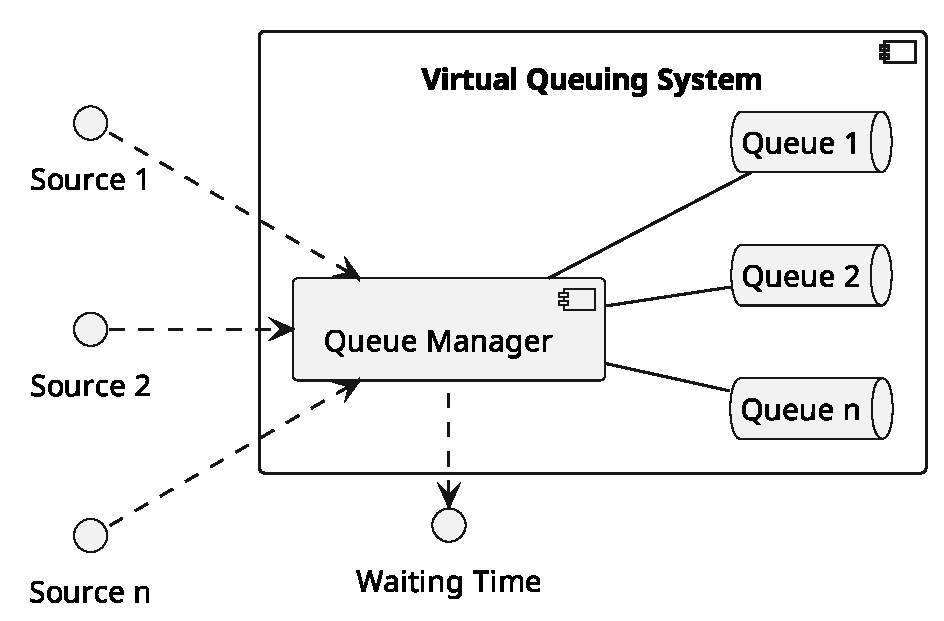
\includegraphics[width=0.6\textwidth]{img/virtual-queuing.eps}
	\caption{Component diagram showing the internal architecture of the \textit{Virtual Queueing} component.
	}
	\label{fig:virtual-queueing-arch}
\end{figure}

\section{Recommender}

\begin{figure}[H]
	\centering
	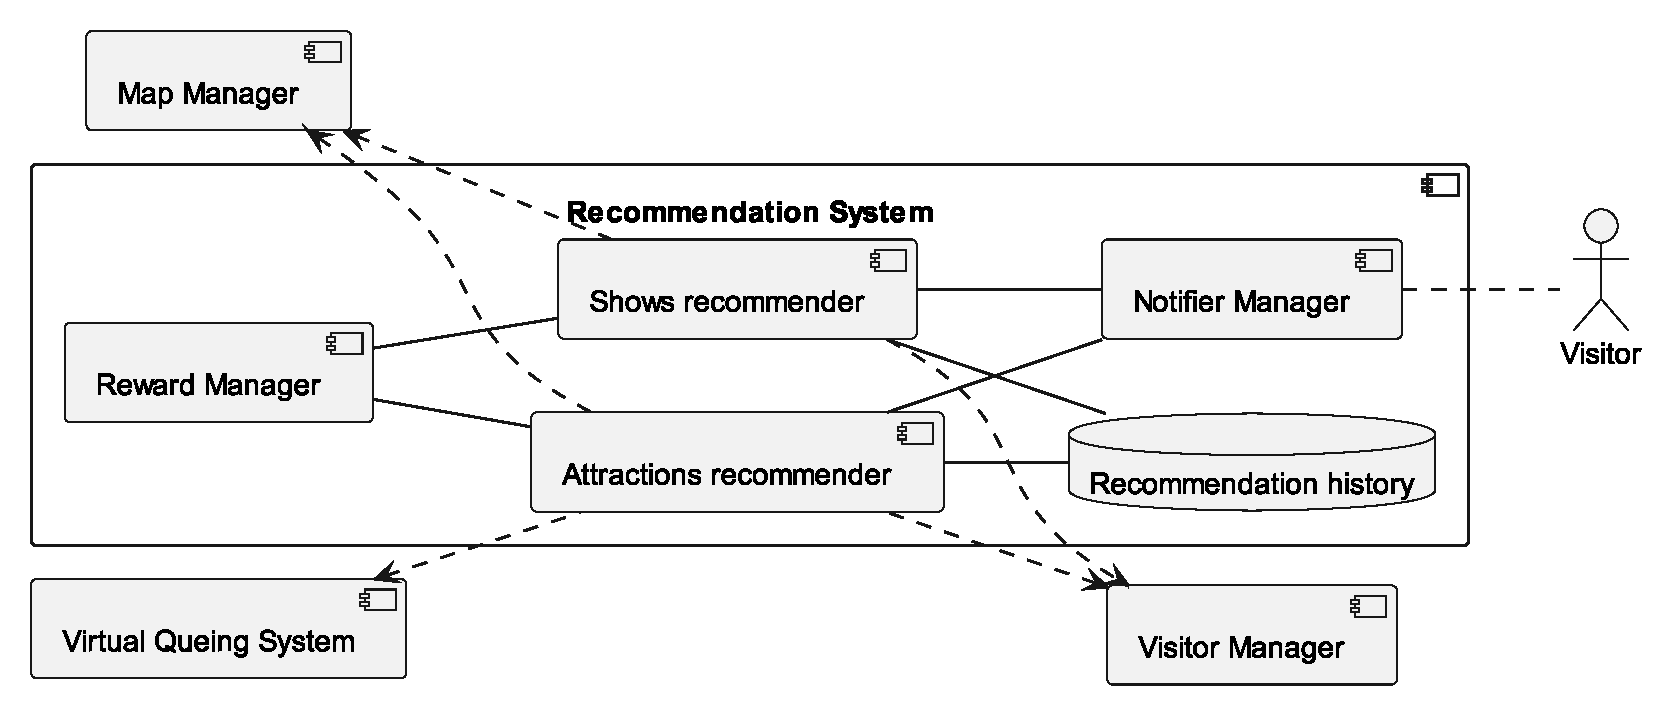
\includegraphics[width=0.9\textwidth]{img/recommender.eps}
	\caption{Component diagram showing the internal architecture of the \textit{Recommender System} component.
	}
	\label{fig:recommender-arch}
\end{figure}

\section{Planner}

\begin{figure}[H]
	\centering
	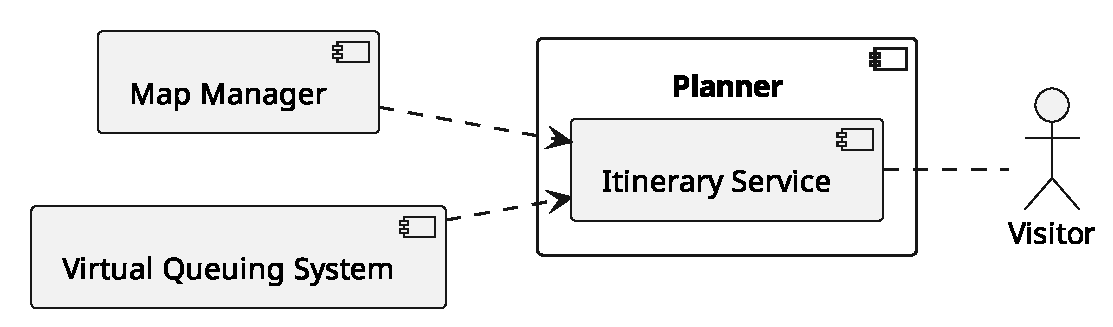
\includegraphics[width=0.7\textwidth]{img/planner.eps}
	\caption{Component diagram showing the internal architecture of the \textit{Planner} component.
	}
	\label{fig:planner-arch}
\end{figure}

\subsection{Sub-GHz Wireless Sensor Network for crowd density estimation}\label{subsec:sub-ghz-wireless-sensor-network-for-crowd-density-estimation}
In our context, crowd density estimation could be advantageous to redirect visitors toward less crowded places within the park.
The classic approach to obtaining this information is to make use of an optical camera-based system but the accuracy of these systems can be
rather dependent on the lighting conditions and they tend to require the availability of a large amount of computing power.
Furthermore, the use of optical cameras raises the spectre of privacy-related issues.
A WSN-based system could potentially be used to simply avoid these issues~\cite{denis2018large}.
In fact, the use of sub-GHz frequencies could be the best decision, due to their increased range and penetration capabilities through objects, walls and human individuals~\cite{denis2018large}.
Moreover, this kind of transceivers, compared to the regular WiFi, have a significant lower power-consumption~\cite{fudickar2014comparing}.

As presented in~\cite{denis2018large}, they managed to show the feasibility of using a sub-GHz wireless network to estimate the
density of large-scale crowds calculating the mean RSS-differences within a WSN between an empty and an active environment and used them
as input to a probabilistic neural network.
Whereas in~\cite{fudickar2014comparing}, showed that Sub GHz transceivers achieve significant lower RSS errors and are less influenced by obstacles attenuations.
Their localisation achieved ca. 1 m more accurate median error distances than the corresponding versions that utilise WiFi transceivers.
In addition, the battery runtimes are extended by 48\% when using Sub GHz transceivers instead of WiFi transceivers.


\section{Visitors Manager}

\begin{figure}[H]
	\centering
	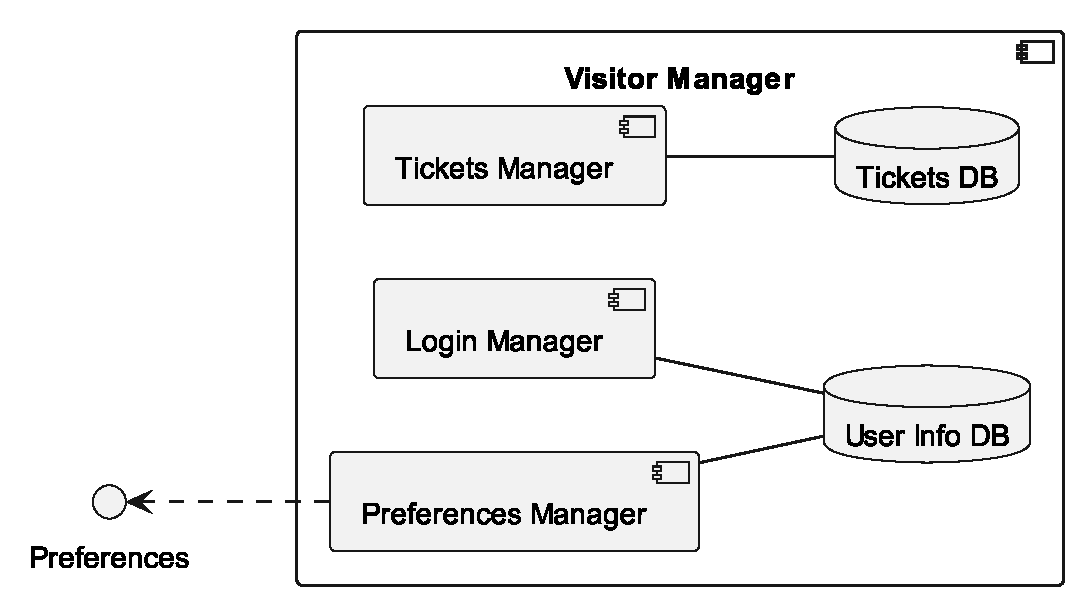
\includegraphics[width=0.7\textwidth]{img/visitor-manager.eps}
	\caption{Component diagram showing the internal architecture of the \textit{Visitor Manager} component.
	}
	\label{fig:visitor-manager-arch}
\end{figure}